
% code profiling and optimization
% 1. difference between slow and fast code
% 2. measuring performance with profilers 
% 2.1 what to measure ?
% 3. gprof
% 4. google perf tools: https://gperftools.github.io/gperftools/cpuprofile.html
% 5. http://www.pixelbeat.org/programming/profiling/
% 6. compiler optimization flags (gcc)
% 6.1. -O, -O1, -O2, -O3 => what changes ?
% 6.2. vectorization (-ftree-vectorize) - how difficult is it to get the vectorizer to engage (what stops vectorization)
% 7. makefile system
% 8. roofline (need to define all terms)

% 9. libraries
% 9.1 sparsesuite
% 9.2 superLU
% 9.3 paradiso
% 9.4 fftw
% 9.5 LAPACK/BLAS
\chapterauthor{Tim Warburton}

\minitoc

\section{Code optimization: profiling}

The first thing we always do when trying to make a code faster is to understand where most of the time is spent during the computation. There are well established tools for serial codes \footnote{There is a very good overview for profiling a CPU code \href{http://euccas.github.io/blog/20170827/cpu-profiling-tools-on-linux.html}{here}.}. For expediency we will use the GNU profiler tool \texttt{\href{https://sourceware.org/binutils/docs/gprof/}{gprof}} to analyze how much time is spent in each of the functions of the reference HW07 kmeans code. 

\subsection{Profiling: preparing the executable}

The first step towards using the \texttt{gprof} tool is to add \texttt{-pg} to the compiler and linker arguments, say via editing the existing \texttt{makefile} by editing the \texttt{CFLAGS} and \texttt{LDFLAGS}  as follows

\begin{minted}{C}
# compiler flags to be used 
CFLAGS = -I$(HDRDIR)  -fopenmp -pg

# link flags to be used             
LDFLAGS = -fopenmp -pg
\end{minted}

In the above we actually also added the \texttt{-fopenmp} flag as we may also use the OpenMP wall clock timer. Performing a \texttt{make clean} and then \texttt{make} again and you should see the following compilation

\begin{tsession}{mytermbg}
\begin{Verbatim}
make 
g++ -I./include  -fopenmp -pg -o src/kmeans.o -c src/kmeans.c 
g++ -I./include  -fopenmp -pg -o src/clusters.o -c src/clusters.c  
g++ -I./include  -fopenmp -pg -o src/data.o -c src/data.c  
g++ -fopenmp  -pg -o kmeans src/kmeans.o src/clusters.o src/data.o -lm 
\end{Verbatim}
\end{tsession} 

By adding the \texttt{-pg} flag we have obliged the compiler to inject extra code into the program that interrupts the code execution to perform statistical sampling of the call stack. With enough samples the profiler can form a reasonable picture of where most of the time is spent during the program execution.

Now that the \texttt{kmeans} executable is instrumented for profiling we can run it as normal as follows

\begin{tsession}{mytermbg}
\begin{Verbatim}
./kmeans data/big_test.dat 100
totalChange = 5.77913
...
totalChange = 1.32544e-09
totalChange = 0
iterations = 16
elapsed = 3.39931
> ls -l
total 2140
drwxrwxr-x 2 tcew tcew    4096 Nov 13 09:51 data
-rw-r--r-- 1 tcew tcew    1843 Nov 13 14:02 gmon.out
...
\end{Verbatim}
\end{tsession} 

If the program finishes execution completely then the profiling library will automatically be called and the \texttt{gmon.out} file is created with profiling information. Unfortunately that file is a binary file and we need to use the \texttt{gprof} tool to interpret the profiling information it contains, which we can do as follows

\begin{tsession}{mytermbg}
\begin{Verbatim}
./kmeans data/big_test.dat 100
gprof ./kmeans |& less
Each sample counts as 0.01 seconds.
  %   cumulative   self              self     total           
 time   seconds   seconds    calls   s/call   s/call  name 
  97.46     1.40     1.40       16     0.09     0.09  clustersAssignDataPoints(clusters_t, data_t)
  2.78      1.44     0.04       16     0.00     0.00  clustersComputeCentroids(clusters_t, data_t)
  0.00      1.44     0.00        1     0.00     0.00  kmeansOutput(data_t, clusters_t, char const*)
  0.00      1.44     0.00        1     0.00     0.00  clusterRandomSetup(int, data_t)
  0.00      1.44     0.00        1     0.00     1.44  kmeans(data_t, clusters_t)
  0.00      1.44     0.00        1     0.00     0.00  dataRead(char const*)
\end{Verbatim}
\end{tsession} 
where we have piped the output from \texttt{gprof} to the \texttt{less} command so that we can scroll through the output at our leisure. Here we show the top part of the profile. It should be immediately obvious that the code is spending a lot of time calling the \texttt{clustersAssignDataPoints}. 

Replacing \texttt{g++} with \texttt{gcc} in the \texttt{makefile}, rebuilding completely, and rerunning we get a new profile

\begin{tsession}{mytermbg}
\begin{Verbatim}
Each sample counts as 0.01 seconds.
%   cumulative   self              self     total           
 time   seconds   seconds    calls   s/call   s/call  name 
 98.89      1.46     1.46       16     0.09     0.09  clustersAssignDataPoints
  1.35      1.48     0.02       16     0.00     0.00  clustersComputeCentroids
  0.00      1.48     0.00        1     0.00     0.00  clusterRandomSetup
  0.00      1.48     0.00        1     0.00     0.00  dataRead
  0.00      1.48     0.00        1     0.00     1.48  kmeans
  0.00      1.48     0.00        1     0.00     0.00  kmeansOutput
\end{Verbatim}
\end{tsession} 

Unlike in the class demos which were performed on my workstation it appears that the GNU C++ and C compilers on Cascades are generating comparable performance codes.

There is definitely some variability in these results. The next step in optimizing this code is to delve into the black box of compiler based optimization.

\subsection{Removing inefficient \texttt{pow} calls}

Some inspection shows that the function calls \texttt{pow} a lot of times to compute the square of some numbers. Removing the calls in HW07 to this function yielded the following profile

\begin{tsession}{mytermbg}
\begin{Verbatim}
Each sample counts as 0.01 seconds.
  %   cumulative   self              self     total           
 time   seconds   seconds    calls  ms/call  ms/call  name    
 97.81      0.80     0.80       16    50.13    50.13  clustersAssignDataPoints
  2.45      0.82     0.02       16     1.25     1.25  clustersComputeCentroids
  0.00      0.82     0.00        1     0.00     0.00  clusterRandomSetup
  0.00      0.82     0.00        1     0.00     0.00  dataRead
  0.00      0.82     0.00        1     0.00   822.09  kmeans
  0.00      0.82     0.00        1     0.00     0.00  kmeansOutput
\end{Verbatim}
\end{tsession} 

We see the time spent in the heavy \texttt{clustersAssignDataPoints} drops by a considerable fraction just by replacing calls to \texttt{pow} with manual  squaring.


\section{Code optimization: compiler flags}

There are several levels of compiler optimizations available that may speed up the execution of your code. The most commonly used compiler flags are \texttt{-O1}, \texttt{-O2}, \texttt{-O3}, \texttt{-Ofast}. The \texttt{-O1} option is the least aggressive in refactoring your code during the compilation phase. The \texttt{-Ofast} is the most aggressive, and in fact violates some IEEE standards on preserving order of operation in some arithmetic expressions. Oddly enough the lesser optimization flags may actually produce a faster executable than some of the more aggressive options. It is easy enough to change the flags, make clean, then make the executable with different options and measure what it does to the execution time.

First we rebuild \texttt{kmeans} with \texttt{-O1} and get this new profile

\begin{tsession}{mytermbg}
\begin{Verbatim}
 %   cumulative   self              self     total           
 time   seconds   seconds    calls  ms/call  ms/call  name    
 93.43      0.27     0.27       16    16.93    16.93  clustersAssignDataPoints
  0.00      0.27     0.00       16     0.00     0.00  clustersComputeCentroids
  0.00      0.27     0.00        1     0.00     0.00  clusterRandomSetup
  0.00      0.27     0.00        1     0.00     0.00  dataRead
  0.00      0.27     0.00        1     0.00   270.95  kmeans
  0.00      0.27     0.00        1     0.00     0.00  kmeansOutput
\end{Verbatim}
\end{tsession} 

The execution time has dropped by more than a factor of three! That's a good return for just editing \texttt{CFLAGS} and \texttt{LDFLAGS} in the \texttt{makefile}.

Using \texttt{-O2} yielded

\begin{tsession}{mytermbg}
\begin{Verbatim}
Each sample counts as 0.01 seconds.
  %   cumulative   self              self     total           
 time   seconds   seconds    calls  ms/call  ms/call  name    
100.39      0.26     0.26       16    16.31    16.31  clustersAssignDataPoints
  0.00      0.26     0.00       16     0.00     0.00  clustersComputeCentroids
\end{Verbatim}
\end{tsession} 

So \texttt{-O1} and \texttt{-O2} are basically similar for this code. The more aggressive \texttt{-O3} and \texttt{-Ofast} options do not change the outcome substantially.  

\section{Comparing performance with different compilers}

So far in this course we have exclusively used the GNU C compiler from the GNU compiler collection. The GNU compilers are open source, distributed without license fees, and ubiquitous since for instance Linux is built using the GNU compilers. However, the GNU compilers are not necessarily best in class on a specific CPU architecture. For the next step in our optimization campaign we switch from using \texttt{gcc} to the Intel using 

\myvbox[mytermbg]{module purge \\ module load intel/18.2}

and edit the \texttt{makefile} compiler flags to use \texttt{icpc} (the Intel C++ compiler) or \texttt{icc} (the Intel C compiler) instead of \texttt{gcc}.
In the next section we summarize the results of using the Intel compiler compared with using the GNU \texttt{gcc} compiler. 

{\bf Note}: we add the  additional command line argument \texttt{-march=native} when using the Intel compiler to instruct it to generate assembler code in the executable specifically for the CPU we are targeting. 

\section{Summary of \texttt{kmeans} optimization study}

In this section we collect together the results from the above study on optimizing the \texttt{kmeans} codes (serial from HW07 and with OpenMP from HW09) to assign the \texttt{HW07/data/big\_test.dat} into one hundred clusters. 

\begin{table}[htbp!]
    \centering
    \begin{tabular}{c|c|c|c|l} \hline
     Code & Experiment & Compiler     & Threads &  Seconds/iteration \\ \hline
     HW07 & Baseline             & \texttt{g++} & 1      & 0.21 \\
     & Switch compiler      & \texttt{gcc} & 1     & 0.21 \\
     & Replace \texttt{pow} & \texttt{gcc} & 1    & 0.052 \\
     & \texttt{-O1}     & \texttt{gcc} & 1    & 0.019 \\
     & \texttt{-O2}     & \texttt{gcc} & 1    & 0.016 \\
     & \texttt{-O3}     & \texttt{gcc} & 1    & 0.016 \\
     & \texttt{-Ofast}  & \texttt{gcc} & 1    & 0.016 \\ 
     & \texttt{-O1 -march=native} & \texttt{icpc} & 1 & 0.016 \\
     & \texttt{-O2 -march=native} & \texttt{icpc} & 1 & 0.0033 \\ \hline
     HW09 & \texttt{-O2 -march=native} & \texttt{icpc} & 1 & 0.0033 \\
     & \texttt{-O2 -march=native} & \texttt{icpc} & 2 & 0.0030 \\
     & \texttt{-O2 -march=native} & \texttt{icpc} & 3 & 0.0021 \\
     & \texttt{-O2 -march=native} & \texttt{icpc} & 4 & 0.0018 \\
      & \texttt{-O2 -march=native} & \texttt{icpc} & 5 & 0.0014 \\
      & \texttt{-O2 -march=native} & \texttt{icpc} & 6 & 0.0011 \\
       & \texttt{-O2 -march=native} & \texttt{icpc} & 7 & 0.0011 \\ \hline
    \end{tabular}     
    \caption{Results from the sequence of experiments performed in the optimization compaign to speed up the \texttt{kmeans} code from HW07 and HW09. }
    \label{kmeansOptimizationResults.tab}
\end{table}

 In Table \ref{kmeansOptimizationResults.tab} we see that just replacing the \texttt{pow} function calls has a very significant impact on the computation time with 4x speed up. Even a modest amount of compiler optimization yields another 3x speed up. Switching from the \texttt{gcc} compiler to the Intel \texttt{icpc} compiler with \texttt{-O2} optimization gives another 2x speed up. Finally, using multi-threading with OpenMP gives another 3x speed up. All of these speed ups are cumulative so we see overall a factor of over 200x speed up which is quite remarkable given that most of the optimizations involved almost zero effort. 
 
 {\bf Note}: the speed up obtained by using OpenMP is rather modest and somewhat disappointing. However, it is important to note that the ``big'' data set only has 100,000 data points and by optimizing the for loops we are running headlong into Amdahl's law. The time taken for the OpenMP fork/join operations and other non-parallel parts of the code will overwhelm the time it takes the threads to complete the optimized parallel threaded loops. To verify this we would increase the number of data points fed to \texttt{kmeans} to increase the ratio of the parallel to serial parts of the code and repeat the strong thread scaling study. This is a fundamental quandary and dilemma for HPC. Highly optimized codes may scale less well than unoptimized codes. In fact you should critically evaluate claims for highly scalable codes that defy the strong limit that Amdahl warns us about.

{\bf Summary}: Overall the speed up obtained in this study are not typical. This is a relatively small code with just a few hot functions. The compiler was able to find optimizations in part because the code is simple and easily refactored. In general you should not expect to see speed ups of this magnitude without investing more effort in a given code.

\iffalse

\newpage
\section{Code optimization: SIMD vectorization}

So far in this course we have focused on parallelism as a way to fully exploit the power of modern CPUs and CPU based clusters like the ARC systems. However, Justin Krometis highlighted a different axis of optimization strategies during his presentation on using parallel libraries in R. He observed that the best speed up for a Monte Carlo sampling algorithm that estimates $\pi$ were obtained when he used so-called vector apply operations in R. This particular optimization delivered much better performance than using the MPI features of Parallel-R or the MPI based features of the Programming Big Data with R (pbdR) library. The key to the vector apply function is that the vector apply operations can be optimized behind the scenes to avoid overheads associate with just-in-time (JIT) compilation and to exploit some special hardware in modern CPUs that we have not explored yet in this course.

\begin{figure}
    \begin{center}
    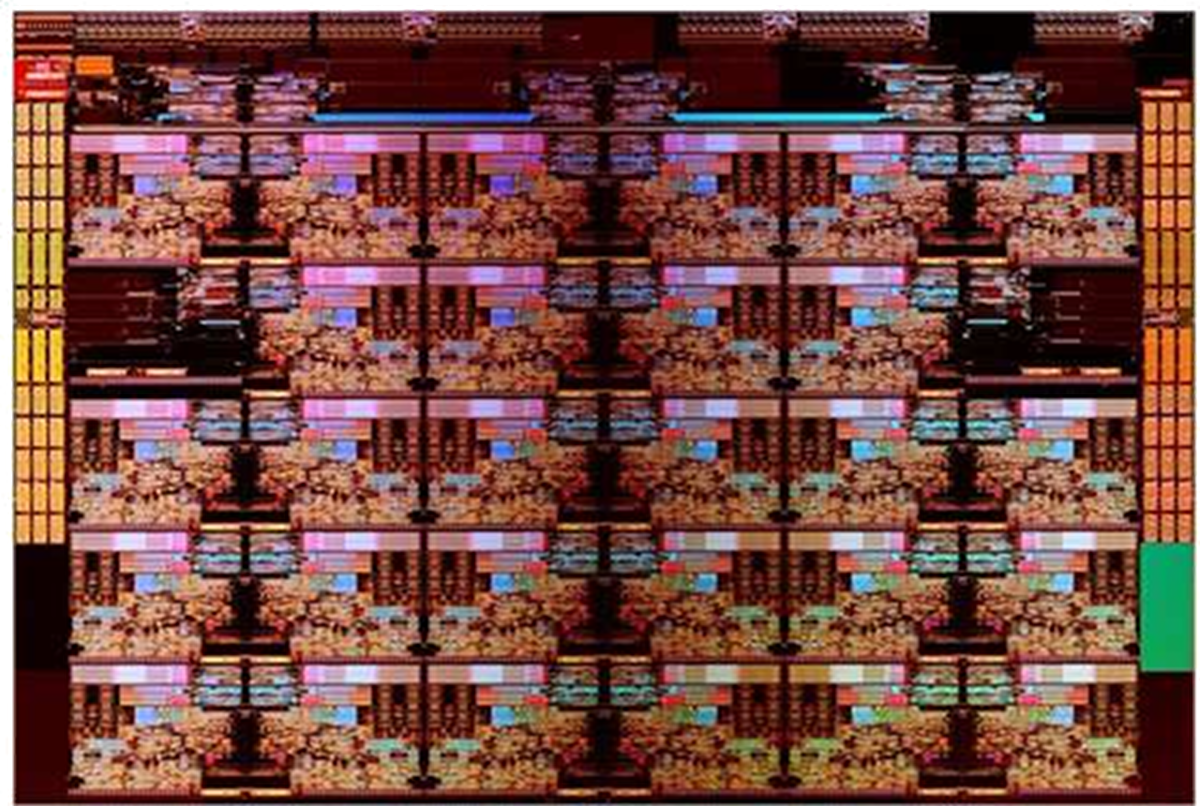
\includegraphics[width=0.45\linewidth]{figures/L14/skylakespxccdieshot.png}
    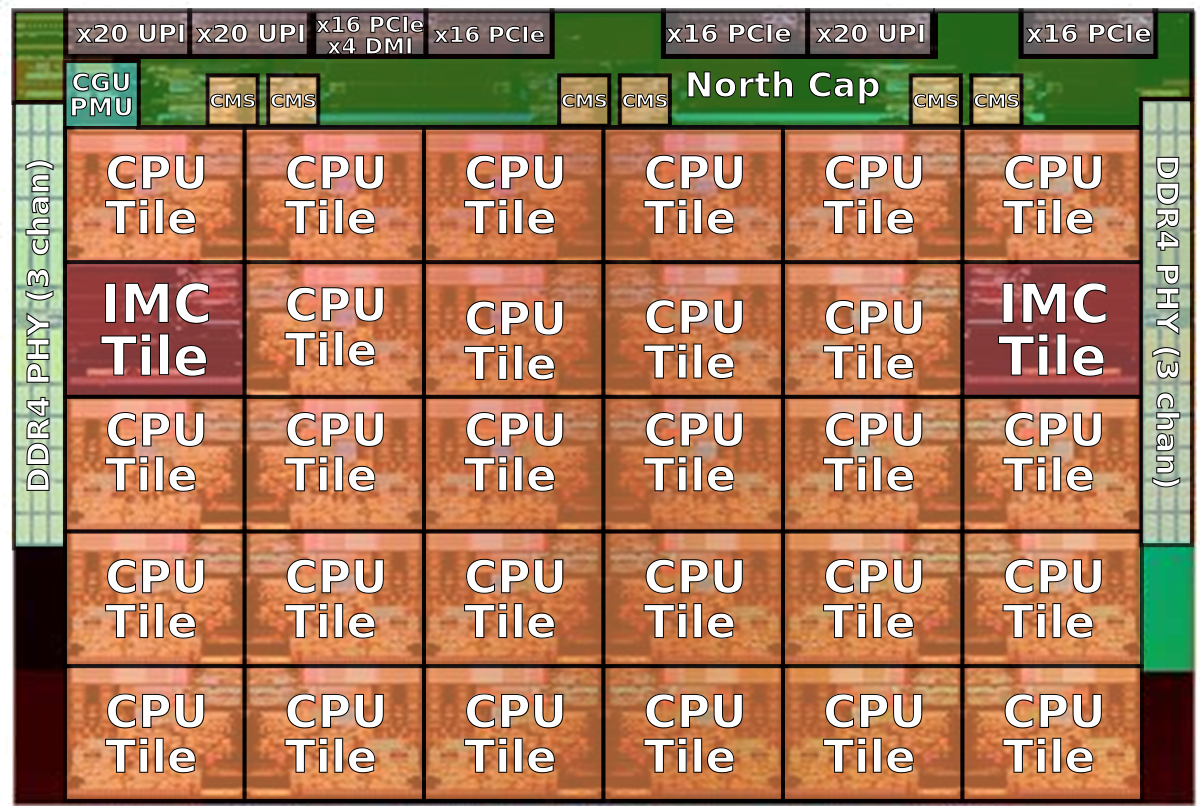
\includegraphics[width=0.45\linewidth]{figures/L14/skylakespxccdieshotannotated.png}
    \end{center}
    \caption{Left: die shot of Intel Xeon 8180. Right: block annotated version. Each CPU core is  labelled as a ``CPU Tile''. The two integrated memory controllers are each labelled as IMC ``Tile''.  Images sourced from \href{https://en.wikichip.org/wiki/File:skylake-sp_xcc_die_shot.png}{https://en.wikichip.org/wiki/File:skylake-sp\_xcc\_die\_shot.png} and \href{https://en.wikichip.org/wiki/File:skylake-sp_xcc_die_shot_(annotated).png}{https://en.wikichip.org/wiki/File:skylake-sp\_xcc\_die\_shot\_(annotated).png}. These images may be copyrighted but are included here under fair usage rights. }
    \label{skylakeDieshotV2.fig}
\end{figure}


To understand what is going on here consider the tiled multi-core architecture of the modern CPUs shown in Figure \ref{skylakeDieshotV2.fig}. We can exploit the multiple cores either by using OpenMP with at least one thread per core, or through MPI with one process per core. Either way we aim to engage more cores in performing parts of a given task. However, there is an additional level of parallelism that we have not yet attempted to exploit: each core is not strictly a serial processing core. Most modern CPU cores include a specialized vector floating point unit that can perform the same operation concurrently with multiple operands. 

\fi 
